\documentclass{article}
\usepackage{graphicx}

\title{TP Calcul Numérique}
\author{Nicolas BOUTON}

\begin{document}

\maketitle

\section*{Cours}

\subsection*{Notations}

\begin{itemize}
\item \textbf{SAXPY} : Scalar a fois X plus Y
\item \textbf{GAXPY} : General matrix A fois X plus Y
\item \textbf{DSL} : Domain Specific Language
\end{itemize}

\section*{Exercice 2}

Nous remarquons 3 chose :

\begin{itemize}
\item Augmentation du conditionnement avec la taille
\item Il faut considéré l'erreur arrière entaché du conditionnement
  pour avoir une approximation des résultats
\item Nous manipulons des algorithmes avec certaines complexité qui
  peuvent être algorithmique ou bien de mémoire
\end{itemize}

\underline{Graphiques :} \newline

Pour l'erreur relative avant :

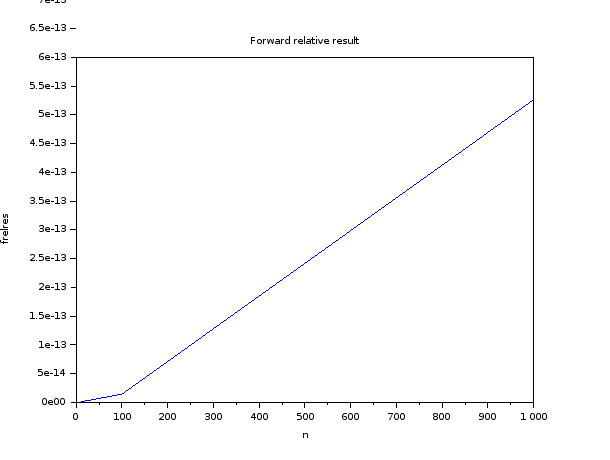
\includegraphics[scale=0.5]{img/frelres.png}

On voit que l'erreur relative avant est très sensible suivant la
taille de la matrice.

\underline{Graphiques :} \newline

Pour l'erreur relative arrière :

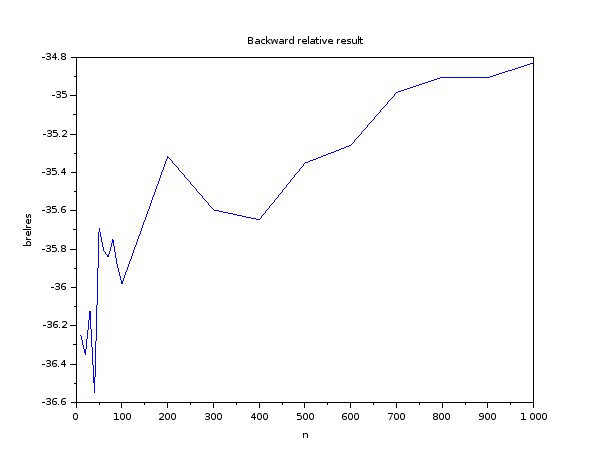
\includegraphics[scale=0.5]{img/brelres.png}

Pour le conditionnement de A :

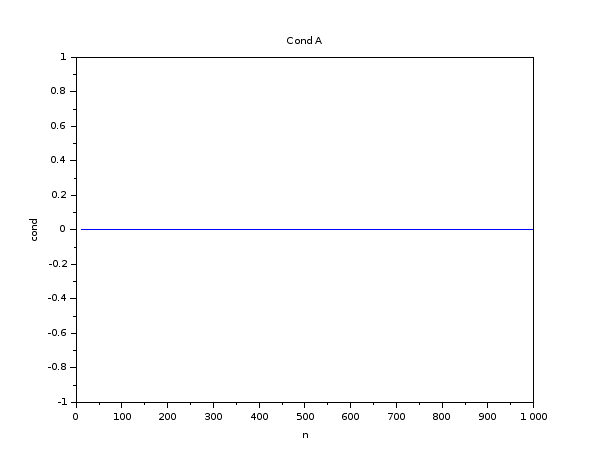
\includegraphics[scale=0.5]{img/capa.png}

Pour les bornes :

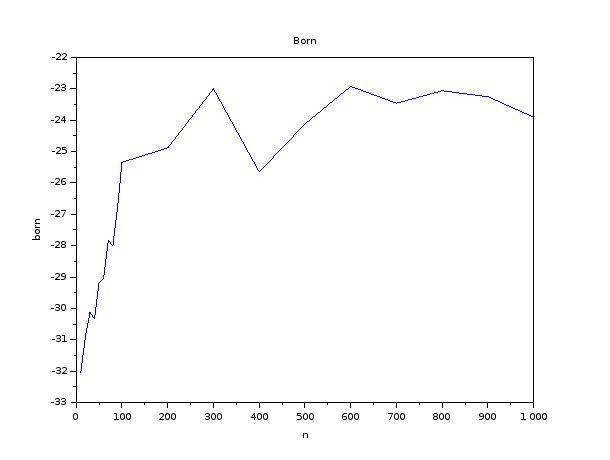
\includegraphics[scale=0.5]{img/born.png}

Nous voyons que pour les autres graphiques la tailles n'influe pas. \newline

Le code source se trouve dans \textbf{exo2.sci}.

\section*{Exercice 3}

Le produit \textbf{matrice x matrice} à une complexité cubique.
Nous remarquons dans un premier temps que l'appel au fonction de
\textbf{Scilab} pour des calculs \textbf{vecteur x vecteur} ou bien
\textbf{vecteur x matrice} au lieu de déroulé nous même les bloucles
est beaucoup plus performant. Il est d'autant plus performant si la
taille des matrices est grandes. \textbf{Scilab} appelle des noyaux de
calcul optimizé tel que blass. \newline

\underline{Graphiques :} \newline

Pour la fonction \textbf{matmat3b} :

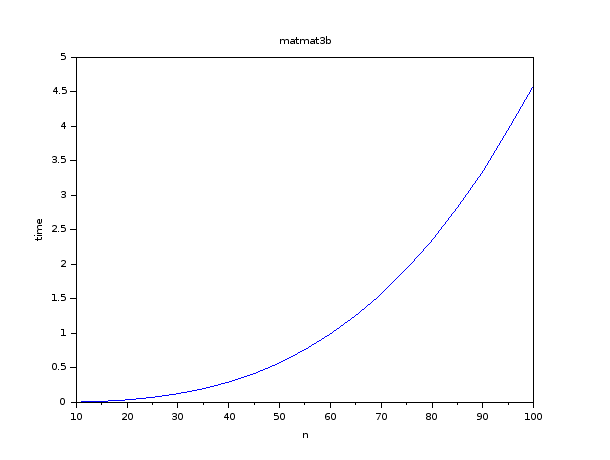
\includegraphics[scale=0.5]{img/matmat3b.png}

On voit que la fonction suit une complexité cubique. \newline

Pour la fonction \textbf{matmat2b} :

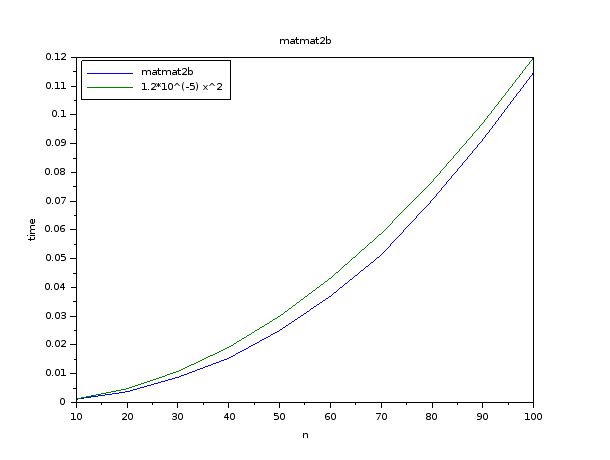
\includegraphics[scale=0.5]{img/matmat2b.png}

On voit que la fonction suit une complexité quadratique. \newline

Pour la fonction \textbf{matmat1b} :

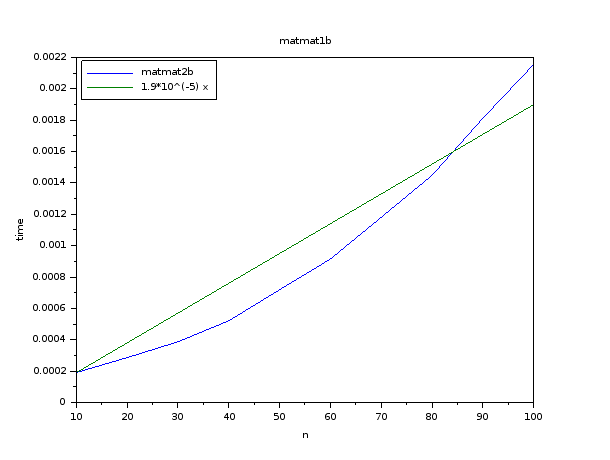
\includegraphics[scale=0.5]{img/matmat1b.png}

On voit que la fonction suit une complexité linéaire.\newline

\begin{itemize}
\item Le code des fonction se trouve dans \textbf{opmat.sci}.
\item Le code de test se trouve dans \textbf{exo3.sci}.
\end{itemize}

\section*{Exercice 4}

\underline{Graphiques :} \newline

Pour l'erreur relative avant pour la matrice supérieure :

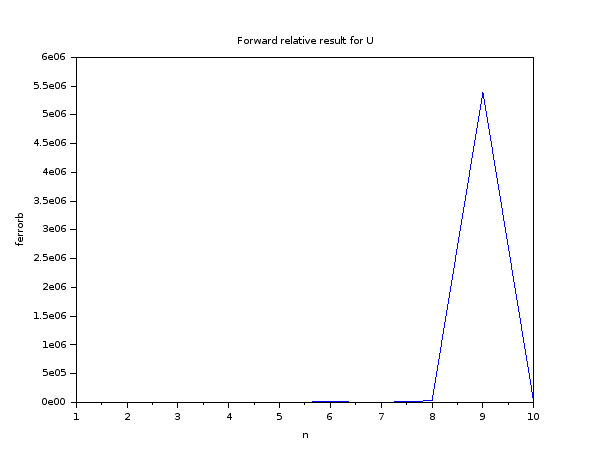
\includegraphics[scale=0.5]{img/U_ferrorb.png}

Pour l'erreur relative arrière pour la matrice supérieure :

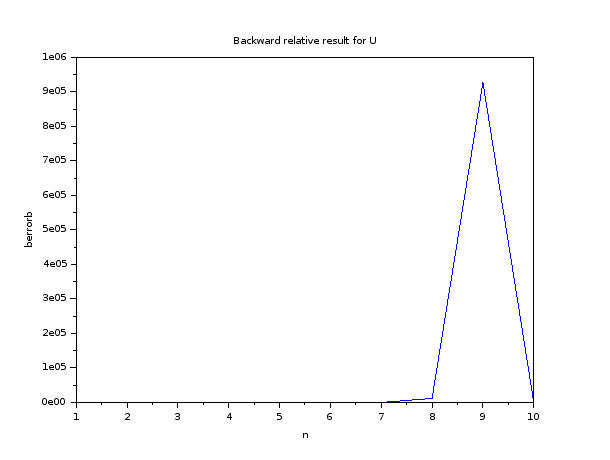
\includegraphics[scale=0.5]{img/U_berrorb.png}

Pour l'erreur relative avant pour la matrice inférieure :

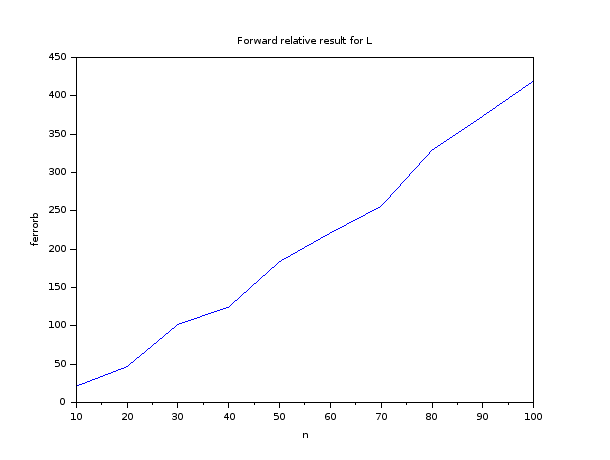
\includegraphics[scale=0.5]{img/L_ferrorb.png}

Pour l'erreur relative arrière pour la matrice inférieure :

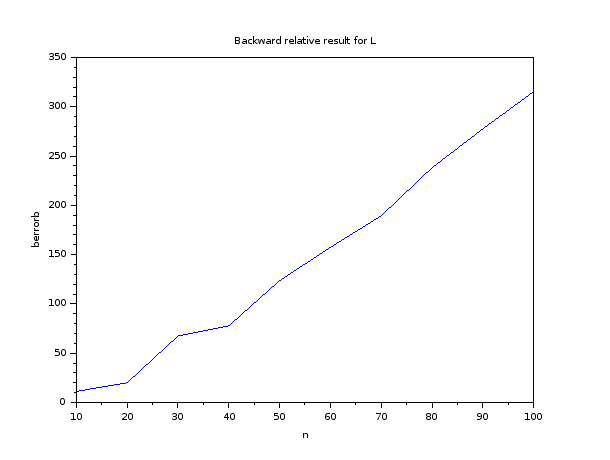
\includegraphics[scale=0.5]{img/L_berrorb.png}

Je ne comprends pas trop ces résultats. Car cela voudrait dire que
l'erreur relative est \textbf{exponentielle} or cela n'a aucun sens.

\section*{Annexe}

Dépot github : https://github.com/Sholde/CN/partie\_2

\end{document}
